\documentclass{llncs}
\usepackage{llncsdoc}

% Bib
\usepackage[square,sort,comma,numbers]{natbib}
\usepackage[nottoc,notlof,notlot]{tocbibind}
\renewcommand\bibname{References}

% Table
\usepackage{array}

\usepackage[english]{babel}
\usepackage[T1]{fontenc}

% utf8
\usepackage[utf8]{inputenc}

% math
\usepackage{amsmath}
\usepackage{mathtools}

\usepackage[toc,page]{appendix}

% lscape.sty Produce landscape pages in a (mainly) portrait document.
\usepackage{lscape}
\usepackage{rotating}

% algorithms
\usepackage[ruled,vlined,linesnumbered]{algorithm2e}
\usepackage{algorithmic}

% float
\usepackage{float}

% graphics
\usepackage{graphicx}
\graphicspath{ {resources/} }

% text components
\usepackage{textcomp}

% euro symbol
\usepackage[official]{eurosym}

\newcommand\myeq{\stackrel{\mathclap{\normalfont\mbox{def}}}{=}}

% page style
\pagestyle{headings}


\newcommand{\keywords}[1]{\par\addvspace\baselineskip
\noindent\keywordname\enspace\ignorespaces#1}

% document settings
\title{Binary Hybrid Particle Swarm Optimization with Wavelet Mutation}

\date{December 21, 2014}
\author{Quang Anh Tran\inst{1} \and Quang Minh Ha\inst{2}
\and Quan Dang Dinh\inst{3} \and Frank Jiang\inst{4}}

\institute{Faculty of Information Technology, Hanoi University, Vietnam\\
\email{anhtq@hanu.edu.vn}
\and
Faculty of Information Technology, Hanoi University, Vietnam\\
\email{minhhq\_fit@hanu.edu.vn}
\and
Faculty of Information Technology, Hanoi University, Vietnam\\
\email{quandd.vnip@gmail.com}
\and
School of Engineering and IT, University of New South Wales, Canberra, Australia\\
\email{F.Jiang@adfa.edu.au}}

% Begin 
\begin{document}


\maketitle

\begin{abstract}
Particle swarm optimization (PSO) is an evolutionary algorithm in which individuals, called particles, move around a multi-dimensional problem space at different directions (trajectories) and speeds (velocities) to find the best solution. A particle movement is based on its previous best result and the previous best result of the entire population. In one of the current PSO variants - HPSOWM \cite{ling2008hybrid}, a mutation process based on wavelet theory was added to the original PSO to prevent premature conclusion of the best solution. This hybrid PSO has improved solution stability and quality over the original algorithm as well as many other hybrid PSO algorithms. However, it is limited to work on a continuous problem space. In this research, we propose a reworked version of HPSOWM which operates on binary-based problem space, and it is called "Binary Hybrid Particle Swarm Optimization with Wavelet Mutation" (BHPSOWM). In this version, the movement mechanism of particles as well as the mutation process are modified and transformed to work with binary element. We conducted an experiment which compare the performance of the binary version of three algorithms: Genetic Algorithm (GA), Particle Swarm Optimization (BPSO) and our proposed algorithm - BHPSOWM. The result showed that our proposed model deliver better performance in terms of the mean cost value, standard deviation and the convergence rate under the same settings.

\keywords{particle swarm optimization, genetic algorithms, binary}
\end{abstract}


\section{Introduction}
% Genetic Algorithms
Among metaheuristic methods, Genetic Algorithm was the first algorithm that utilizes the power of biological mechanisms, and more specifically, the power of natural selection and evolution. It was firstly introduced by Holland in the 1970s \cite{holland1992genetic}. In this algorithm, starting from an initial population of chromosomes (which are bits that compose the program), a proportion of the best of them are selected, based on a fitness function, to create a new population. Those selected chromosomes are then enter a reproduction (or recombination) process where more than one of them are used to produce a new child solution. The children are then chosen with probability for mutation process, where one or some genes in a chromosome are changed from its initial state to maintain the genetic diversity. Finally we have a new population and the process continues until we reach the optimal solution or time/memory limits.

Genetic Algorithms can provide a good approximation of the solution of all types of problems and it has been successfully applied in many problems including scheduling, optimization of networks, engineering, rule discovery \ldots \cite{ross1994applications}

Where GA was influenced by the biological mechanisms, another evolutionary algorithm called Particle Swarm Optimization (PSO) which is introduced by Kennedy and Eberhard in 1995 \cite{kennedy2010particle}, simulates the the movement of organisms in a bird flock or fish school. It was initially used as an optimization technique for use in real-number problem spaces \cite{kennedy1997discrete}. Since its creation, there have been many variants which were proposed. They mostly focus on tuning the velocity of the particle, to balance between local search and global search \cite{shi1998modified}\cite{clerc2002particle}. In 1997, Kennedy and Eberhart modified PSO into a binary search space version. They tested with De Jong's five test functions \cite{de1975analysis} and concludes that binary PSO is capable of solving these problems rapidly. 

In this research, we adapt many ideas from binary PSO implementation to propose a binary version of Hybrid PSO with Wavelet Mutation (HPSOWM), which is the work of \cite{ling2008hybrid} to solve continuous search space. When HPSOWM was proven to outweigh other approaches (HPSOM \cite{esmin2005hybrid}, HGAPSO \cite{juang2004hybrid}, HGPSO \cite{noel2004simulation}) in finding optimal solution, convergence rate \ldots, it hasn't been tested in binary version yet. That is the purpose of this research, to implement binary version of HPSOWM, to evaluate its performance against GA and binary PSO (BSPO) using many different benchmark test functions which are divided into three categories of different characteristics.

This paper is organized as follows: the first section gives the introduction. The second section discusses the backgrounds of this research which are PSO and HPSOWM. Next we discuss about how to transform those two algorithms from continuous to binary version. After that, we describe the experiment with settings, benchmark functions and analyze the results. Finally a conclusion is given with the overall result of this proposed model.

\section{Backgrounds}
\subsection{Particle Swarm Optimization (PSO)}
PSO is an algorithm that simulates the sociological behavior of bird flocking. In the search space, we define a swarm $X$, which has many particles $x^p(t) \in \{x^1(t), x^2(t), \ldots, \gamma\}$ where $\gamma$ is a number of particles and $t$ is the $t$th iteration among $T$ total iterations. Each particle $x^p$ consists of many elements, $x^p_i$ where $i = 1,2,3, \ldots, \kappa$, with $\kappa$ is the dimension of a particle.

Firstly, the particles of the swarm are initialized and evaluated by a predefined fitness function. The objective of the PSO is to minimize these fitness function values. In order to move the particle in the search space, a velocity $v^p_j(t)$ is defined. It is the flight speed of the $j$th element of the $p$th particle at the $t$th iteration. Additionally, $x^p_j(t)$ is the current position of that element. The velocity and current position is then calculated by the following formulae:
\begin{equation}
v_{j}^{p}(t) = 2 \cdot rand() \cdot (pbest_{j}^{p} - x_{j}^{p}(t-1))
+ 2 \cdot rand() \cdot (gbest_{j} - x_{j}^{p}(t-1))
\end{equation}

\begin{equation}
x^p_j(t) = x^p_j(t - 1) + v^p_j(t)
\end{equation}

Another improved version of PSO which is introduced in \cite{eberhart2000comparing}, added two factors: the constriction and inertia which change the velocity calculation to:

\begin{equation}
v_{j}^{p}(t) = k \cdot \{w \cdot v^p_j(t-1) + \varphi_1 \cdot rand() \cdot (pbest_{j}^{p} - x_{j}^{p}(t-1))
+ \varphi_2 \cdot rand() \cdot (gbest_{j} - x_{j}^{p}(t-1)) \}
\end{equation}

where $k$ is the constriction factor and $w$ is the inertia factor, $\varphi_1$ and $\varphi_2$ are constants.

Even with the improved version of PSO, when the particle coincides with the global best position, the particle will move away from this point if the two factors above are different from zero. Furthermore, the particles will stop moving when their velocities are close to zero and they catch up with the global best position. This phenomena is called $stagination$ \cite{eberhart1998comparison}. To overcome this phenomena, the mutation process of GA has been added to PSO to form up a Hybrid PSO with Mutation (HPSOM). We will discuss this mutation process among with the Wavelet Mutation in the next section.

\subsection{Hybrid PSO with Wavelet Mutation}
The initial version of PSO with mutation process works as follows: a random particle is selected to be moved to another position in the search space by using mutation under the following operation:
\begin{equation}
mut(x_j) = x_j - \omega, r < 0
\end{equation}
\begin{equation}
mut(x_j) = x_j + \omega, r \geq 0
\end{equation}
where $x_j$ is a randomly chosen element of the particle above, $\omega$ is randomly generated in the range of $[0, 0.1 x (para^j_{max} - para^j_{min})]$, $r$ is a random number between +1 and -1, $para^j_{max}$ and $para^j_{min}$ are the upper and lower bounds of each particle element. Therefore, we can see that $\omega$ represents $1/10$ of the search space.

This version of PSO can overcome the $stagination$ phenomena. However, it can easily be seen that the mutating space is fixed by $\omega$. It is not always the best strategy for using the same size mutation space all the time. Therefore, in \cite{ling2008hybrid}, the author proposed an improvement method to dynamically adjust the mutating size $\omega$ based on the wavelet theory as follows.

\subsubsection{Hybrid PSO with Wavelet Mutation}
\
Each particle element has a chance to mutate which is controlled by a probability of mutation $p_m \in [0, 1]$. For each element, we generate a random number between 0 and 1 $r$, if $r \leq p_m$, the mutation will take place on that element. In details, let $x^p(t) = [x^p_1(t), x^p_2(t), \ldots, x^p_k(t)]$ be the current selected particle, with $x^p_j(t)$ is its randomly chosen element, $x^p_j(t) \in [param^j_{min}, param^j_{min}]$. After the mutation process, the resulting particle is $\bar{x}^p(t)$

\[ \bar{x}^p(t) = \left\{ \begin{array}{ll}
         x^p_j(t) + \sigma \times (para^j_{max} - x^p_j(t)) & \mbox{if $\sigma > 0$} \\
        x^p_j(t) + \sigma \times (x^p_j(t) - para^j_{min}) & \mbox{if $\sigma \leq 0$}.\end{array} \right. \] 

where $j \in 1,2,3, \ldots k$ is the dimension of the particle and:
\begin{equation}
	\sigma = \frac{1}{\sqrt{a}}\psi(\frac{\varphi}{a})
\end{equation}

where $\psi(x)$ is a wavelet - a continuous time function (see Figure \ref{fig:fig1}) represents a certain seismic signal that satisfies two properties:

\begin{equation}
	\int_{-\infty}^{+\infty}\psi(x)dx = 0
\end{equation}

and

\begin{equation}
	\int_{-\infty}^{+\infty}|\psi(x)|^2dx < 0
\end{equation}

\begin{figure} [H]
\centering
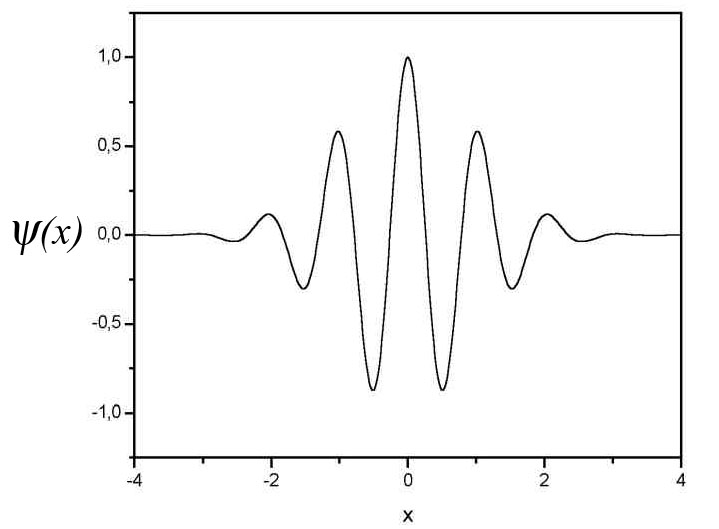
\includegraphics[width=60.72mm]{resources/morlet1}
\caption{The original form of the Morlet wavelet}\label{fig:fig1}
\end{figure}

In this paper, we adapt this approach (HPSOWM) and transform the real-valued particles into binary-based ones. This will be discussed in the next section.

\section{From PSO, HPSOWM to BPSO, BHPSOWM}
A binary-based particle consists of a bit string in which each element can take a value of one or zero. Such particle ``moves'' by flipping a number of its bits from 0 to 1 and vice versa. A velocity vector composed of bits could be used to modify a binary particle. However, applying formula (\ref{eq:formula1}) in a binary space by replacing $v^p$, $pbest^p$ and $gbest$ with bit strings would actually make the particle move randomly around the problem space, not following any direction. The reason for this is that flipping a bit from 0 to 1 means taking a full jump from the lower bound to the upper bound.

What would be the velocity for a binary-based particle? How trajectory should be understood in a binary problem space? These two questions can be answered by defining the values in the velocity vector as ``\emph{probabilities that a bit will take value 1 or 0}''. Such probability value is used in the following way:

\begin{verbatim}
if (rand() < probability) then
    x = value1;
else
    x = value2;
\end{verbatim}

Note that the $rand()$ function returns a real number $x$ such that $ 0 \leq x < 1$.

Thus, the velocity vector $v^p$ must be scaled down to real numbers in the range $[0.0, 1.0]$ and $x_j^p$ will take either 0 or 1 as value. Specifically, the velocity value, which is between 0.0 and 1.0, will be compared to a random number in the same range. If it is higher than the random value,$x_j^p$ will take value 1, otherwise $x_j^p$ will take value 0. Note that in the original version of PSO, the magnitudes on the dimensions of velocity vector are limited by their dynamic range, which can be quite large. The rate at which the velocity increases or decreases is also high. To address this problem, a logistic function -- the sigmoid function -- was used to scale down the velocity values. The function is as follow:

\begin{equation} \label{eq:formula3}
S(t) = \frac{1}{(1 + e^{-t})}
\end{equation}

With the sigmoid function, we can keep the old velocity update formula (\ref{eq:formula1}). This function makes sure it generates a number between 0.0 and 1.0 from any real number $t$. This property eliminates the need of a $v^{max}$ value which was used in the original version to limit the particle speed to about one tenth of the search space's length. With the new definition of velocity and the sigmoid function, now particles are updated using the following logic instead of formula (\ref{eq:formula2}):

\begin{equation} \label{eq:formula4}
x_j^p =
\begin{cases}
1, & rand() < S(v_j^p)\\
0, & rand() > S(v_j^p)
\end{cases}
\end{equation}

This transformation makes the particles move more slowly on each dimension towards the two best values. As a result, one bit would change from 0 to 1 before another does, whereas previously, many bits would flip at the same time due to using a bit string as a velocity vector. This approach allows the particles to scan the problem space much more carefully, reducing the risk of ``stepping over'' a good solution.

Trajectory in a binary space can now be explained. In a continuous space, the direction of the velocity vector decides the particle's trajectory. As a particle moves closer to the global best position, its coordinates get closer to the coordinates of $gbest$. In a binary space, the ``position'' of a particle is actually defined by the velocity vector, which contains probabilities. A particle is said to be close to another particle when the probabilities of corresponding bits are close to each other. One interesting thing about this algorithm is that, even when two particles are at the same position they could result in different bit strings thanks to the random value in the particle update process described in (\ref{eq:formula4}). Note that with a probability value of 0.9, there is still a 10\% chance that a bit would be 0.

\section{Experiments \& Results}
\subsection{Benchmark functions}
In this paper, we compare the performance of the binary version of GA, PSO and HPSOWM that will be called BGA, BPSO, BHPSOWM respectively, using a suite of benchmark test functions (shown in \ref{table1}). Many different kinds of optimization problems are covered by these benchmark test functions \cite{ling2008hybrid}. They are divided into three categories as follows:
\begin{itemize}
	\item Category I - Unimodal functions: a symmetry model with a single minimum. Function $f_1$ to $f_7$ are in this category
	\item Category II - Multimodal functions with few local minima. Function $f_8$ to $f_{13}$ belong to this.
	\item Category III - Multimodal functions with many local minima which includes function $f_{14}$ to $f_{18}$
\end{itemize}


% Benchmark functions

\begin{table}[H]\label{table1}
	\caption{Benchmark test functions}
	\begin{center}
		\bgroup
		\def\arraystretch{1.5}%  1 is the default, change whatever you need
	    \begin{tabular}{  >{\centering\arraybackslash}m{8cm} | >{\centering\arraybackslash}m{3cm} | >{\centering\arraybackslash}m{3cm} }
		    \hline
		    Test function & Domain range & Optimal point \\ \hline
    
		    $f_1(x) = \sum\limits_{i=1}^{30}{x_i}^2$ & 
		    $-100 \leq x_i \leq 100$ & 
		    $f_i(0) = 0$ 
    			\\ \hline
    			
    			$f_2(x) = \sum\limits_{i=1}^{9}\Big[ 100(x_{i+1} - x_{i}^2)^2 + (x_i - 1)^2 \Big]$ &
    			$-2.048 \leq x_i \leq 2.048$ &
    			$f_2(1) = 0$    			
    			\\ \hline
    			
    			$f_3(x) = \sum\limits_{i=1}^{100}(|x_i + 0.5|)^2$ &
    			$-10 \leq x_i \leq 10$ &
    			$f_3(0) = 0$ 
    			\\ \hline    			
    			
    			$f_4(x) = \sum\limits_{i=1}^{10}ix_{i}^4 + random[0,1)$ &
    			$-2.56 \leq x_i \leq 2.56$ &
    			$f_4(0) = 0$
    			\\ \hline
    			
    			$f_5(x) = max{|x_i|, 1 \leq i \leq 30}$ &
    			$-100 \leq x_i \leq 100$ &
    			$f_5(0) = 0$
    			\\ \hline
    			
    			$f_6(x) = \sum\limits_{i=1}^{30}|x_i| + \prod\limits_{i=1}^{30}|x_i|$ &
    			$-10 \leq x_i \leq 10$ &
    			$f_5(0) = 0$
    			\\ \hline
    			
    			
    			$f_7(x) = -cos(x_1) \cdot cos(x_2) \cdot exp \Big( -\Big( (x_1 - \pi)^2 + (x_2 + \pi)^2\Big) \Big)$ &
    			$-300 \leq x_1, x_2 \leq 300$ &
    			$f_7(\Big[ \pi,\pi \Big]) = -1$
    			\\ \hline
    			
    			$f_8(x) = \Bigg[ \frac{1}{500} + \sum\limits_{j=1}^{25}\frac{1}{j + \sum_{i=1}^{2}(x_i - a_{ij})^6} \Bigg]^{-1}$ &
    			$-65.536 \leq x_1, x_2 \leq 65.536$ &
    			$f_8(|-32, 32|) \approx 1$
    			\\ \hline
    			
    			$f_9(x) = \sum\limits_{i=1}^{9} \Bigg[ a_i - \frac{x_1(b_{i}^2 + b_i x_2)}{b_{i}^2 + b_i x_3 + x_4} \Bigg]^2$ &
    			$-5 \leq x_i \leq 5$ &
    			$f_9(0.1928, 0.1928, 0.1231, 0.1358) \approx 0.0003075$
    			\\ \hline
    			
    			$f_{10}(x) = -\frac{sin(x_1)sin(x_2)}{x_1 x_2}$ &
    			$-10 \leq x_1, x_2 \leq 10$ &
    			$\displaystyle\lim_{x \to |0,0|}f_{10}(x) = -1$
    			\\ \hline
    			
    			$f_{11}(x) = 4x_{1}^2 - 2.1x_{1}^4 + \frac{1}{3}x_{1}^6 + x_1 x_2 - 4x_{2}^2 + 4x_{2}^4$ &
    			$-5 \leq x_1, x_2 \leq 5$ &
    			$f_{11}(\Big[ 0.08983, -0.7126 \Big]) = f_{11}(\Big[ -0.08983, 0.7126 \Big]) \approx -1.0316$
    			\\ \hline
    			
    			$f_{12}(x) = -\sum\limits_{i=1}^{30}c_i exp\Bigg[ -\sum\limits_{j=1}^{3}a_{ij}\Big( x_j - p_{ij} \Big)^2 \Bigg]$ &
    			$0 \leq x_i \leq 1$ &
    			$f_{12}(0.114, 0.556, 0.852) \approx -3.8628$
    			\\ \hline
    			
    			$f_{13}(x) = -\sum\limits_{i=1}^{4}c_i exp\Bigg[ -\sum\limits_{j=1}^{6}a_{ij}\Big( x_j - p_{ij} \Big)^2 \Bigg]$ &
    			$0 \leq x_i \leq 1$ &
    			$f_{13}(\Big[ 0.201, 0.15, 0.477, 0.275, 0.311, 0.627 \Big]) \approx -3.32$
    			\\ \hline
    			
			$
			f_{14}(x) = 0.1 \left\{ \begin{array}{l}
        			sin^2(\pi 3 x_1) \\
        			+ \sum\limits_{i=1}^{29}(x_i - 1)^2 \cdot \Big[ 1 + sin^2(3 \pi x_{i+1}) \Big] \\
        			+ (x_30 - 1)^2 \Big[ 1 + sin^2(2 \pi x_30) \Big]
    			\end{array}\right\}    		
    			+ \sum\limits_{i=1}^{30}u(x_i, 5, 100, 4)
			$ &
			$-50 \leq x_i \leq 50$ &
			$f_{14}(1) = 0$
			\\ \hline
			
			$f_{15}(x) = \sum\limits_{i=1}^{30}\Bigg[ x_{i}^2 - 10 cos(2\pi x_i) + 10 \Bigg]$ &
			$-50 \leq x_i \leq 50$ &
			$f_{15}(0) = 0$
			\\ \hline
			
			$f_{16}(x) = \frac{1}{4000}\sum\limits_{i=1}^{30}x_{i}^2 - \prod_{i=1}^{30}cos\Bigg( \frac{x_i}{\sqrt{i}} \Bigg) + 1$ &
			$-600 \leq x_i \leq 600$ &
			$f_{16}(0) = 0$
			\\ \hline
			
			$f_{17}(x) = -20exp \Bigg( -0.2\sqrt{\frac{1}{30}\sum\limits_{i=1}^{30}x_{i}^2} \Bigg) - exp \Bigg( \frac{1}{30} \sum\limits_{i=1}^{30}cos 2 \pi x_i \Bigg) + 20 + e$ &
			$-32 \leq x_i \leq 32$ &
			$f_{17}(0) = 0$
			\\ \hline
			
			$f_{18}(x) = -\sum\limits_{i=1}^{10}\Bigg( x_i sin\Bigg( \sqrt{|x_i|} \Bigg) \Bigg)$ &
			$-500 \leq x_i \leq 500$ &
			$f_{18}([420.9687, \cdots 420.9687]) = -10 \times 418.9829 = -4189.829$
			\\ \hline
    			
    		\end{tabular}
    		\egroup
	\end{center}
\end{table}

\subsection{Experiment settings}
We adapt the settings from the original research of HPSOWM \cite{ling2008hybrid} which has some main settings are:
\begin{itemize}
	\item Swarm size: 50
	\item Number of runs: 50
	\item Time limit for each run: 120 seconds
	\item The probability of crossover for GA: 0.001
	\item The initial population: we start from a single initial population so we can compare the performance among three algorithms starting from the same point
\end{itemize}
As of the binary version, we also adapt the settings from \cite{kennedy1997discrete} as:
\begin{itemize}
	\item $V_{max}$ which is the maximum value for the velocity is set to 6
\end{itemize}

\subsection{Results and Discussions}

- Compare BHPSOWM with BPSO and GA \\
- Use benchmark functions in three categories: unimodal functions, multimodal functions with few local minima, multimodal functions with many local minima \\
- Experiment settings \\
- Show convergence table \\
- Show result table with Standard Deviation, ... \\



\begin{table}[H]
\caption{Comparison between BHPSOWM, BPSO and GA - Category I: unimodal functions}\label{tab:graph1}
  \begin{tabular*}{\textwidth}{cc}
    \begin{tabular}[c]{@{}c@{}}
    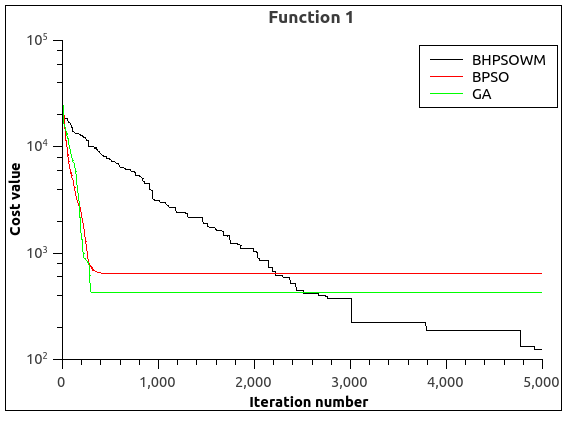
\includegraphics[width=60mm]{resources/f1_graph} \\
    $f_1(x)$
    \end{tabular}
    &
    \begin{tabular}[c]{@{}c@{}}
    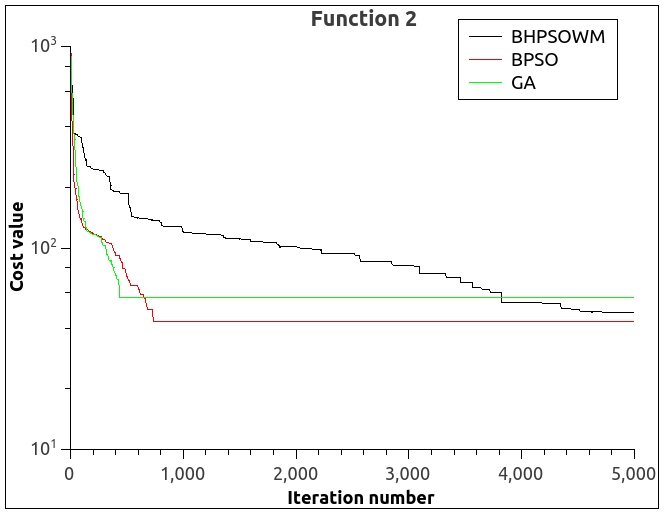
\includegraphics[width=60mm]{resources/f2_graph} \\
    $f_2(x)$
    \end{tabular}
    \\
    \begin{tabular}[c]{@{}c@{}}
    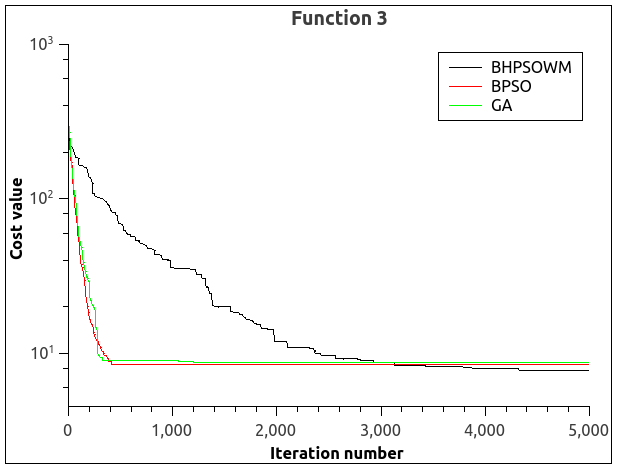
\includegraphics[width=60mm]{resources/f3_graph} \\
    $f_3(x)$
    \end{tabular}
    &
    \begin{tabular}[c]{@{}c@{}}
    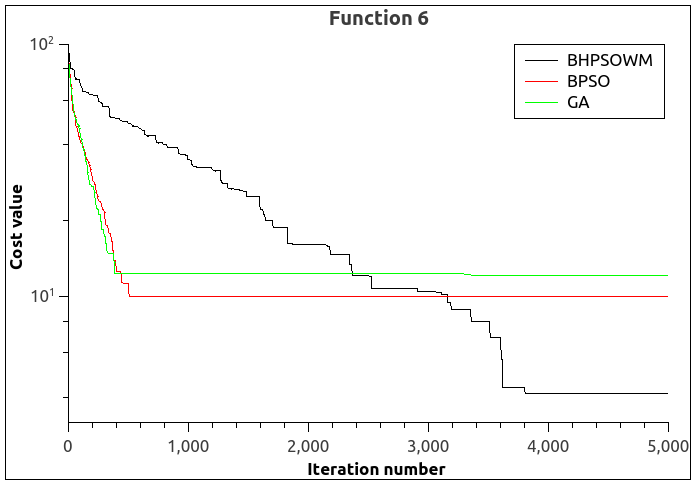
\includegraphics[width=60mm]{resources/f6_graph} \\
    $f_6(x)$
    \end{tabular}
    
    \\
  \end{tabular*}
\end{table}


\begin{table}[H]
\caption{Comparison between BHPSOWM, BPSO and GA - Category II: multimodal functions with few local minima}\label{tab:graph2}
  \begin{tabular*}{\textwidth}{cc}
    \begin{tabular}[c]{@{}c@{}}
    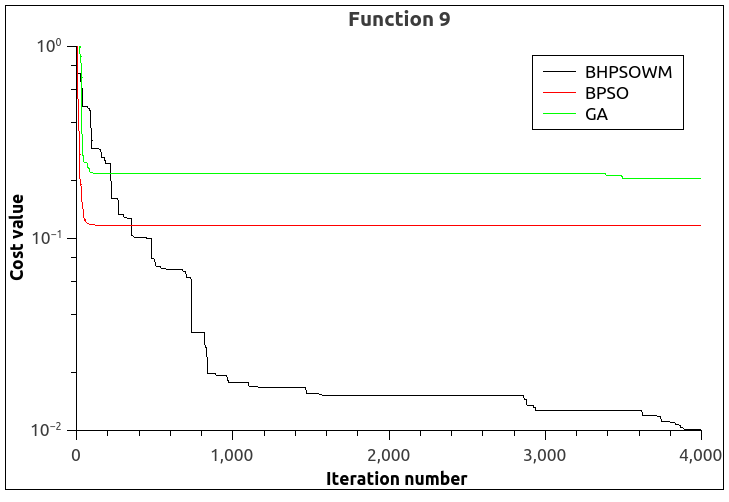
\includegraphics[width=60mm]{resources/f9_graph} \\
    $f_9(x)$
    \end{tabular}
    &
    \begin{tabular}[c]{@{}c@{}}
    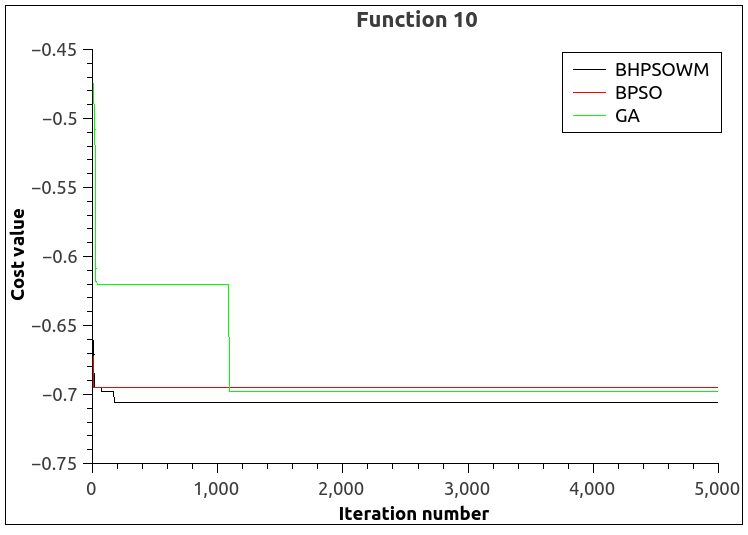
\includegraphics[width=60mm]{resources/f10_graph} \\
    $f_10(x)$
    \end{tabular}
    \\
    \begin{tabular}[c]{@{}c@{}}
    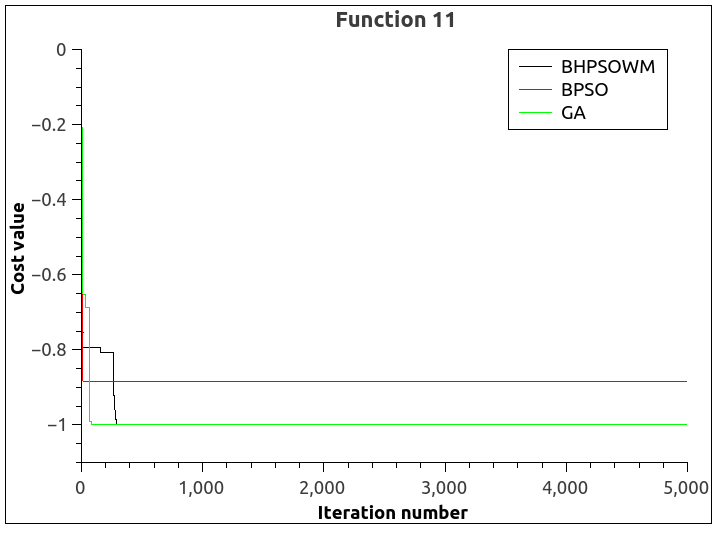
\includegraphics[width=60mm]{resources/f11_graph} \\
    $f_11(x)$
    \end{tabular}
    &
    \begin{tabular}[c]{@{}c@{}}
    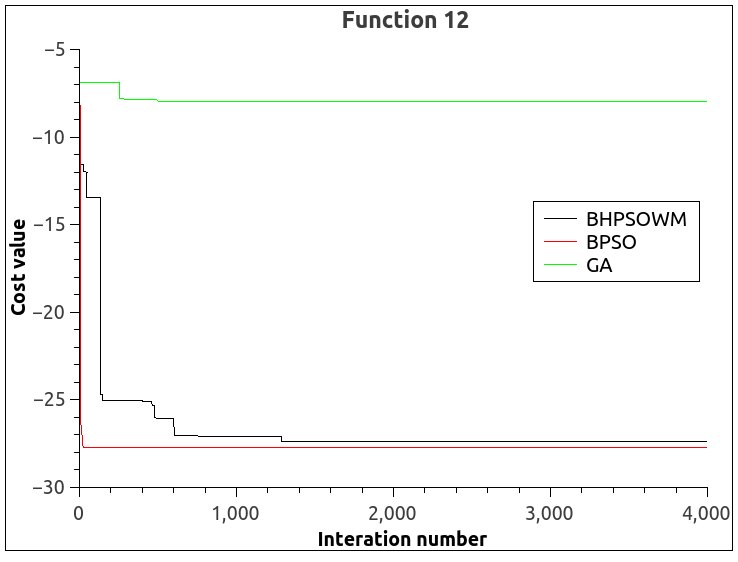
\includegraphics[width=60mm]{resources/f12_graph} \\
    $f_12(x)$
    \end{tabular}
    \\
    \begin{tabular}[c]{@{}c@{}}
    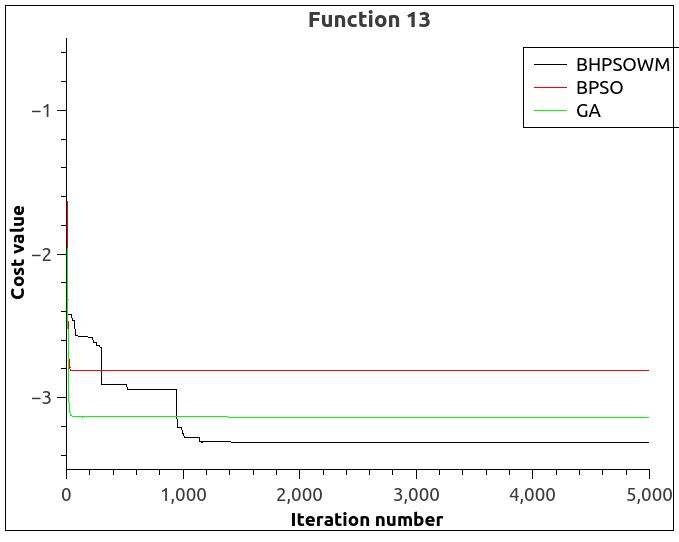
\includegraphics[width=60mm]{resources/f13_graph} \\
    $f_13(x)$
    \end{tabular}
    &

    \\
  \end{tabular*}
\end{table}


\begin{table}[H]
\caption{Comparison between BHPSOWM, BPSO and GA - Category III: multimodal functions with many local minima}\label{tab:graph3}
  \begin{tabular*}{\textwidth}{cc}
    \begin{tabular}[c]{@{}c@{}}
    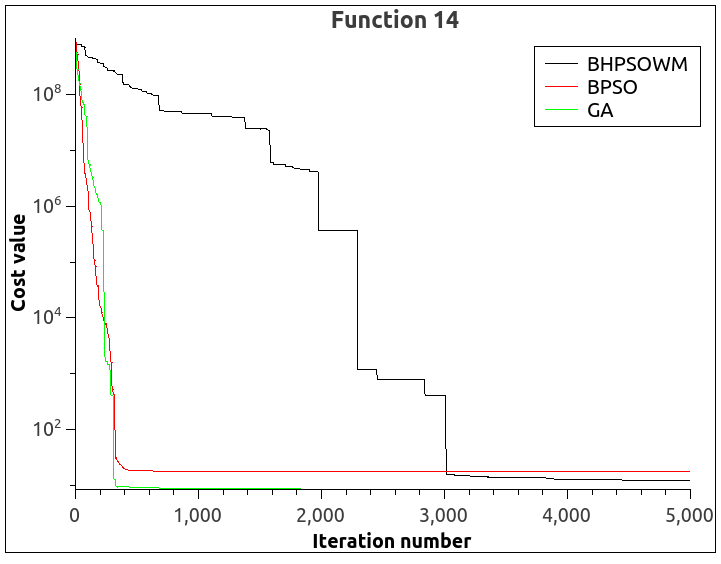
\includegraphics[width=60mm]{resources/f14_graph} \\
    $f_14(x)$
    \end{tabular}
    &
    \begin{tabular}[c]{@{}c@{}}
    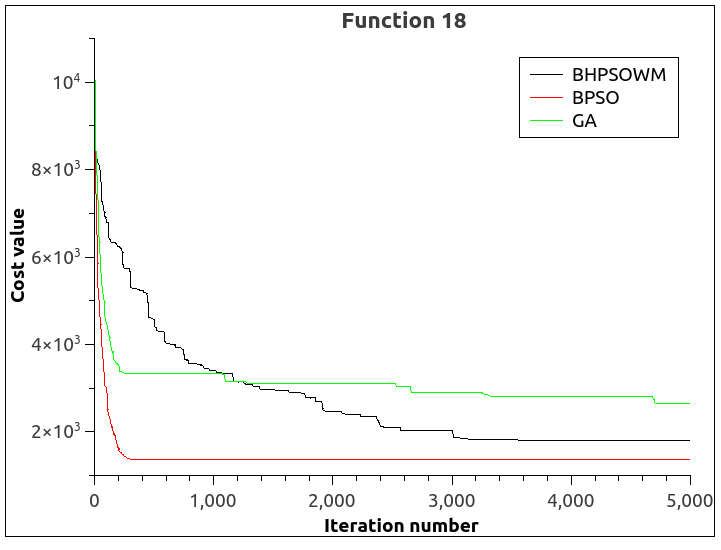
\includegraphics[width=60mm]{resources/f18_graph} \\
    $f_18(x)$
    \end{tabular}

    \\
  \end{tabular*}
\end{table}





\renewcommand{\arraystretch}{1}
\setlength{\tabcolsep}{.1em}
\begin{table}[H]
\caption{Comparison between BHPSOWM, BPSO and GA with benchmark testing function - Category I}\label{tab:tb2}
\centering
  \begin{tabular}{|c|l|r|r|r|}
  \hline
  & & BHPSOWM & BPSO & GA \\
  \hline
  
  % begin function
  \begin{tabular}[c]{@{}c@{}}
  $f_1(x)$\\
  $T = 120$
  \end{tabular}
  &
  \begin{tabular}[c]{@{}lll@{}}
  Best\\
  Mean\\
  Std Dev
  \end{tabular}
  &
  \begin{tabular}{@{}rrr@{}}
  0.000\\
  0.000\\
  0.000
  \end{tabular}
  &
  \begin{tabular}{@{}rrr@{}}
  0.000\\
  0.000\\
  0.000
  \end{tabular} 
  &
  \begin{tabular}{@{}rrr@{}}
  0.000\\
  0.000\\
  0.000
  \end{tabular} 
  \\ \hline
  % end of function 
  
  % begin function
  \begin{tabular}[c]{@{}c@{}}
  $f_2(x)$\\
  $T = 120$
  \end{tabular}
  &
  \begin{tabular}[c]{@{}lll@{}}
  Best\\
  Mean\\
  Std Dev
  \end{tabular}
  &
  \begin{tabular}{@{}rrr@{}}
  0.000\\
  0.000\\
  0.000
  \end{tabular}
  &
  \begin{tabular}{@{}rrr@{}}
  0.000\\
  0.000\\
  0.000
  \end{tabular} 
  &
  \begin{tabular}{@{}rrr@{}}
  0.000\\
  0.000\\
  0.000
  \end{tabular} 
  \\ \hline
  % end of function 
  
  % begin function
  \begin{tabular}[c]{@{}c@{}}
  $f_3(x)$\\
  $T = 120$
  \end{tabular}
  &
  \begin{tabular}[c]{@{}lll@{}}
  Best\\
  Mean\\
  Std Dev
  \end{tabular}
  &
  \begin{tabular}{@{}rrr@{}}
  0.000\\
  0.000\\
  0.000
  \end{tabular}
  &
  \begin{tabular}{@{}rrr@{}}
  0.000\\
  0.000\\
  0.000
  \end{tabular} 
  &
  \begin{tabular}{@{}rrr@{}}
  0.000\\
  0.000\\
  0.000
  \end{tabular} 
  \\ \hline
  % end of function 
  
  % begin function
  \begin{tabular}[c]{@{}c@{}}
  $f_4(x)$\\
  $T = 120$
  \end{tabular}
  &
  \begin{tabular}[c]{@{}lll@{}}
  Best\\
  Mean\\
  Std Dev
  \end{tabular}
  &
  \begin{tabular}{@{}rrr@{}}
  0.000\\
  0.000\\
  0.000
  \end{tabular}
  &
  \begin{tabular}{@{}rrr@{}}
  0.000\\
  0.000\\
  0.000
  \end{tabular} 
  &
  \begin{tabular}{@{}rrr@{}}
  0.000\\
  0.000\\
  0.000
  \end{tabular} 
  \\ \hline
  % end of function 
  
  % begin function
  \begin{tabular}[c]{@{}c@{}}
  $f_5(x)$\\
  $T = 120$
  \end{tabular}
  &
  \begin{tabular}[c]{@{}lll@{}}
  Best\\
  Mean\\
  Std Dev
  \end{tabular}
  &
  \begin{tabular}{@{}rrr@{}}
  0.000\\
  0.000\\
  0.000
  \end{tabular}
  &
  \begin{tabular}{@{}rrr@{}}
  0.000\\
  0.000\\
  0.000
  \end{tabular} 
  &
  \begin{tabular}{@{}rrr@{}}
  0.000\\
  0.000\\
  0.000
  \end{tabular} 
  \\ \hline
  % end of function 
  
  % begin function
  \begin{tabular}[c]{@{}c@{}}
  $f_6(x)$\\
  $T = 120$
  \end{tabular}
  &
  \begin{tabular}[c]{@{}lll@{}}
  Best\\
  Mean\\
  Std Dev
  \end{tabular}
  &
  \begin{tabular}{@{}rrr@{}}
  0.000\\
  0.000\\
  0.000
  \end{tabular}
  &
  \begin{tabular}{@{}rrr@{}}
  0.000\\
  0.000\\
  0.000
  \end{tabular} 
  &
  \begin{tabular}{@{}rrr@{}}
  0.000\\
  0.000\\
  0.000
  \end{tabular} 
  \\ \hline
  % end of function 
  
  % begin function
  \begin{tabular}[c]{@{}c@{}}
  $f_7(x)$\\
  $T = 120$
  \end{tabular}
  &
  \begin{tabular}[c]{@{}lll@{}}
  Best\\
  Mean\\
  Std Dev
  \end{tabular}
  &
  \begin{tabular}{@{}rrr@{}}
  0.000\\
  0.000\\
  0.000
  \end{tabular}
  &
  \begin{tabular}{@{}rrr@{}}
  0.000\\
  0.000\\
  0.000
  \end{tabular} 
  &
  \begin{tabular}{@{}rrr@{}}
  0.000\\
  0.000\\
  0.000
  \end{tabular} 
  \\ \hline
  % end of function  
  
  \end{tabular}
\end{table}










\renewcommand{\arraystretch}{1}
\setlength{\tabcolsep}{.1em}
\begin{table}[H]
\caption{Comparison between BHPSOWM, BPSO and GA with benchmark testing function - Category II}\label{tab:tb3}
\centering
  \begin{tabular}{|c|l|r|r|r|}
  \hline
  & & BHPSOWM & BPSO & GA \\
  \hline
  
  % begin function
  \begin{tabular}[c]{@{}c@{}}
  $f_8(x)$\\
  $T = 120$
  \end{tabular}
  &
  \begin{tabular}[c]{@{}lll@{}}
  Best\\
  Mean\\
  Std Dev
  \end{tabular}
  &
  \begin{tabular}{@{}rrr@{}}
  0.000\\
  0.000\\
  0.000
  \end{tabular}
  &
  \begin{tabular}{@{}rrr@{}}
  0.000\\
  0.000\\
  0.000
  \end{tabular} 
  &
  \begin{tabular}{@{}rrr@{}}
  0.000\\
  0.000\\
  0.000
  \end{tabular} 
  \\ \hline
  % end of function  
  
  % begin function
  \begin{tabular}[c]{@{}c@{}}
  $f_9(x)$\\
  $T = 120$
  \end{tabular}
  &
  \begin{tabular}[c]{@{}lll@{}}
  Best\\
  Mean\\
  Std Dev
  \end{tabular}
  &
  \begin{tabular}{@{}rrr@{}}
  0.000\\
  0.000\\
  0.000
  \end{tabular}
  &
  \begin{tabular}{@{}rrr@{}}
  0.000\\
  0.000\\
  0.000
  \end{tabular} 
  &
  \begin{tabular}{@{}rrr@{}}
  0.000\\
  0.000\\
  0.000
  \end{tabular} 
  \\ \hline
  % end of function  
  
  % begin function
  \begin{tabular}[c]{@{}c@{}}
  $f_10(x)$\\
  $T = 120$
  \end{tabular}
  &
  \begin{tabular}[c]{@{}lll@{}}
  Best\\
  Mean\\
  Std Dev
  \end{tabular}
  &
  \begin{tabular}{@{}rrr@{}}
  0.000\\
  0.000\\
  0.000
  \end{tabular}
  &
  \begin{tabular}{@{}rrr@{}}
  0.000\\
  0.000\\
  0.000
  \end{tabular} 
  &
  \begin{tabular}{@{}rrr@{}}
  0.000\\
  0.000\\
  0.000
  \end{tabular} 
  \\ \hline
  % end of function  
  
  % begin function
  \begin{tabular}[c]{@{}c@{}}
  $f_11(x)$\\
  $T = 120$
  \end{tabular}
  &
  \begin{tabular}[c]{@{}lll@{}}
  Best\\
  Mean\\
  Std Dev
  \end{tabular}
  &
  \begin{tabular}{@{}rrr@{}}
  0.000\\
  0.000\\
  0.000
  \end{tabular}
  &
  \begin{tabular}{@{}rrr@{}}
  0.000\\
  0.000\\
  0.000
  \end{tabular} 
  &
  \begin{tabular}{@{}rrr@{}}
  0.000\\
  0.000\\
  0.000
  \end{tabular} 
  \\ \hline
  % end of function  
  
  % begin function
  \begin{tabular}[c]{@{}c@{}}
  $f_12(x)$\\
  $T = 120$
  \end{tabular}
  &
  \begin{tabular}[c]{@{}lll@{}}
  Best\\
  Mean\\
  Std Dev
  \end{tabular}
  &
  \begin{tabular}{@{}rrr@{}}
  0.000\\
  0.000\\
  0.000
  \end{tabular}
  &
  \begin{tabular}{@{}rrr@{}}
  0.000\\
  0.000\\
  0.000
  \end{tabular} 
  &
  \begin{tabular}{@{}rrr@{}}
  0.000\\
  0.000\\
  0.000
  \end{tabular} 
  \\ \hline
  % end of function  
  
  % begin function
  \begin{tabular}[c]{@{}c@{}}
  $f_13(x)$\\
  $T = 120$
  \end{tabular}
  &
  \begin{tabular}[c]{@{}lll@{}}
  Best\\
  Mean\\
  Std Dev
  \end{tabular}
  &
  \begin{tabular}{@{}rrr@{}}
  0.000\\
  0.000\\
  0.000
  \end{tabular}
  &
  \begin{tabular}{@{}rrr@{}}
  0.000\\
  0.000\\
  0.000
  \end{tabular} 
  &
  \begin{tabular}{@{}rrr@{}}
  0.000\\
  0.000\\
  0.000
  \end{tabular} 
  \\ \hline
  % end of function  
  
  \end{tabular}
\end{table}













\renewcommand{\arraystretch}{1}
\setlength{\tabcolsep}{.1em}
\begin{table}[H]
\caption{Comparison between BHPSOWM, BPSO and GA with benchmark testing function - Category III}\label{tab:tb4}
\centering
  \begin{tabular}{|c|l|r|r|r|}
  \hline
  & & BHPSOWM & BPSO & GA \\
  \hline
  
  % begin function
  \begin{tabular}[c]{@{}c@{}}
  $f_14(x)$\\
  $T = 120$
  \end{tabular}
  &
  \begin{tabular}[c]{@{}lll@{}}
  Best\\
  Mean\\
  Std Dev
  \end{tabular}
  &
  \begin{tabular}{@{}rrr@{}}
  0.000\\
  0.000\\
  0.000
  \end{tabular}
  &
  \begin{tabular}{@{}rrr@{}}
  0.000\\
  0.000\\
  0.000
  \end{tabular} 
  &
  \begin{tabular}{@{}rrr@{}}
  0.000\\
  0.000\\
  0.000
  \end{tabular} 
  \\ \hline
  % end of function  
  
  
  % begin function
  \begin{tabular}[c]{@{}c@{}}
  $f_15(x)$\\
  $T = 120$
  \end{tabular}
  &
  \begin{tabular}[c]{@{}lll@{}}
  Best\\
  Mean\\
  Std Dev
  \end{tabular}
  &
  \begin{tabular}{@{}rrr@{}}
  0.000\\
  0.000\\
  0.000
  \end{tabular}
  &
  \begin{tabular}{@{}rrr@{}}
  0.000\\
  0.000\\
  0.000
  \end{tabular} 
  &
  \begin{tabular}{@{}rrr@{}}
  0.000\\
  0.000\\
  0.000
  \end{tabular} 
  \\ \hline
  % end of function  
  
  % begin function
  \begin{tabular}[c]{@{}c@{}}
  $f_16(x)$\\
  $T = 120$
  \end{tabular}
  &
  \begin{tabular}[c]{@{}lll@{}}
  Best\\
  Mean\\
  Std Dev
  \end{tabular}
  &
  \begin{tabular}{@{}rrr@{}}
  0.000\\
  0.000\\
  0.000
  \end{tabular}
  &
  \begin{tabular}{@{}rrr@{}}
  0.000\\
  0.000\\
  0.000
  \end{tabular} 
  &
  \begin{tabular}{@{}rrr@{}}
  0.000\\
  0.000\\
  0.000
  \end{tabular} 
  \\ \hline
  % end of function  
  
  % begin function
  \begin{tabular}[c]{@{}c@{}}
  $f_17(x)$\\
  $T = 120$
  \end{tabular}
  &
  \begin{tabular}[c]{@{}lll@{}}
  Best\\
  Mean\\
  Std Dev
  \end{tabular}
  &
  \begin{tabular}{@{}rrr@{}}
  0.000\\
  0.000\\
  0.000
  \end{tabular}
  &
  \begin{tabular}{@{}rrr@{}}
  0.000\\
  0.000\\
  0.000
  \end{tabular} 
  &
  \begin{tabular}{@{}rrr@{}}
  0.000\\
  0.000\\
  0.000
  \end{tabular} 
  \\ \hline
  % end of function  
  
  % begin function
  \begin{tabular}[c]{@{}c@{}}
  $f_18(x)$\\
  $T = 120$
  \end{tabular}
  &
  \begin{tabular}[c]{@{}lll@{}}
  Best\\
  Mean\\
  Std Dev
  \end{tabular}
  &
  \begin{tabular}{@{}rrr@{}}
  0.000\\
  0.000\\
  0.000
  \end{tabular}
  &
  \begin{tabular}{@{}rrr@{}}
  0.000\\
  0.000\\
  0.000
  \end{tabular} 
  &
  \begin{tabular}{@{}rrr@{}}
  0.000\\
  0.000\\
  0.000
  \end{tabular} 
  \\ \hline
  % end of function  
  \end{tabular}
\end{table}

\section{Conclusions}
In this paper, we adapt the idea HPSOWM to build a binary version - BHPSOWM. This transforms the approach from a continuous problem into a discrete problem. The proposed approach is then used to compare with other two binary algorithms: GA and BPSO. We conducted an experiment using 18 benchmark functions that falls into three main categories (unimodal, multimodal few local minima, multimodal many local minima), using the same parameters from previous research of HPSOWM and BPSO. The result proves the preservation of the advantages of HPSOWM in providing good and stable solutions with steady convergence rate and small standard deviation among all tests. It also showed that BHPSOWM outperformed GA and BPSO in 9/18 functions, has the same performance in 5/18 functions and be a runner-up in the rest 4 functions.

However, even providing better goodness and stability, the convergence rate of BHPSOWM is slower than GA and BPSO, this is also the inspiration for us to work in the future researches.

\section{Acknowledgements}
This research was fully supported by the Vietnam National Foundation for Science and Technology Development (NAFOSTED) under project number 102.01-2012.04

% bibliography
\bibliographystyle{bibliography}
\bibliography{bibliography}
%\nocite{*}

\end{document}